%
%
%
\documentclass[twoside]{wiss}

\usepackage{graphicx}
\usepackage{nidanfloat} %% appended in WISS2010 for Future Vision (2010/7/7:akita)
\usepackage{multicol}
\usepackage{here} % [H]とするとその場所に配置されるらしい
\usepackage{color}


\usepackage{listings}
\definecolor{lightgray}{rgb}{.9,.9,.9}
\definecolor{darkgray}{rgb}{.4,.4,.4}
\definecolor{purple}{rgb}{0.65, 0.12, 0.82}

\lstdefinelanguage{JavaScript}{
  keywords={typeof, new, true, false, catch, function, return, null, catch, switch, var, if, in, while, do, else, case, break},
  keywordstyle=\color{blue}\bfseries,
  ndkeywords={class, export, boolean, throw, implements, import, this, .},
  ndkeywordstyle=\color{darkgray}\bfseries,
  identifierstyle=\color{black},
  sensitive=false,
  comment=[l]{//},
  morecomment=[s]{/*}{*/},
  commentstyle=\color{purple}\ttfamily,
  stringstyle=\color{red}\ttfamily,
  morestring=[b]',
  morestring=[b]"
}

\lstset{
   language=JavaScript,
   backgroundcolor=\color{white},
   extendedchars=true,
   basicstyle=\footnotesize\ttfamily,
   showstringspaces=false,
   showspaces=false,
   numbers=left,
   numberstyle=\footnotesize,
   numbersep=5pt,
   tabsize=2,
   breaklines=true,
   showtabs=false,
   captionpos=b,
   basewidth={0.5em,0.4em}
}

%% balance.styを追加 (2012/9/27:watanabe, Igarashi)
\usepackage{balance}    %% 最後のページの高さを揃えるために追加  (2012/9/27:watanabe, Igarashi)
%%% 最後のページの2段組の高さを揃える.\balanceを入れる.
%%% そろえたくないときは,\nobalance

% \usepackage{authblk}

\journalhead{Babascript}

\begin{document}

\title{Babascript: 人とコンピュータの協調による処理実行環境}
\etitle{} %2012年では英文タイトルは廃止されました.記入しないでください

\author{{馬場匠見} \hspace{1em}
        {橋本翔} \hspace{1em}
        {増井俊之
        \affil{慶應義塾大学大学院政策・メディア研究科, 慶應義塾大学環境情報学部}}
        }

\begin{abstract}
プログラムに人力処理を簡単に組み込むことのできるシステム「Babascript」を提案する。
Babascriptは、シンプルな人力処理命令構文と、命令に対する返り値を返せるスマートフォンアプリケーションを組み合わせることで実現する、プログラム上で人力処理を実現するための仕組みである。
Babascriptでは、通常のプログラムにおける関数呼び出しと同じ記法で人への処理を命令することができる。
人とコンピュータがプログラム上で協調して動作していくことによって、
コンピュータだけでは実現しなかった処理の実現や人の行動そのもののプログラム化が可能となる。
その具体的な応用例として、「仕事のプログラム化」と「人を使った実世界プログラミング」について示す。
\end{abstract}

\maketitle

\section{はじめに}
コンピュータには処理が困難なタスクであっても、人ならば処理できることがある。
例えば、その場の雰囲気を数値化・文字列化することはコンピュータには処理は困難だが、人なら処理可能だ。
このような、コンピュータだけでは実現が困難な処理を実現するために、人を計算資源として利用する手法はヒューマンコンピュテーション\cite{humancomputation}と呼ばれ、様々な研究が行われている。

% ここ直す
人の処理能力は有用であり、人力処理をプログラムから扱うことが出来れば、コンピュータだけでは実現しなかった処理を実現することができる。
しかし、既存のプログラミング言語の処理実行対象はコンピュータであるため、人に対する処理命令構文は含まれていない。
プログラムから人力処理を利用できるようにする技術は、クラウドソーシング等の分野において研究が進んでいる(\cite{automan}, \cite{crowddb}, \cite{crowdforge}等)。
クラウドソーシングは、インターネットを経由して不特定多数の群衆にタスク処理を依頼する手法だ\cite{riseofcrowdsourcing}。

プログラムから人力処理を実行するためには、既存の手法ではクラウドソーシングプラットフォームの利用が必要となる。
そのため、例えば、家族や職場の人、研究室のメンバーのような、特定の人物をプログラムに組み込み、処理実行命令を送るといったことは困難だ。
また、処理命令の記法も複雑である。
既存の研究事例では、クラウドソーシングプラットフォームへのアクセスキーや複雑な設定を記述したり、SQL文のようなものをプログラム上に直接記述するといった記法のものが存在する。
これらの事例では、記法が複雑化することが多く、シンプルな記述で実装することはできない。

以上のような問題をふまえ、本論文では、Babascriptプログラミング環境について述べる。
% この文どうにかする
Babascript環境は、関数呼び出しによって人に処理命令の通知ができるBabascript(プログラム例 図\ref{script_01})と、
Babascriptからの命令を受け取り、処理結果を入力することのできるスマートフォン向けwebアプリケーションのBabascript Client(図\ref{webapp-interface})から構成される。
Babascript環境では、特定の人物を実行対象とするため、クラウドソーシングプラットフォームを利用しない。
Babascript環境によって、既存のプログラミング言語上で人への処理命令を、通常のプログラムにおける関数呼び出しとほぼ同じ記述で実現できる。

本論文ではBabascript環境の応用の例として、「仕事のプログラム化」と「人を使った実世界プログラミング」について述べる。
% どんな時に使えるのかを述べる

% プログラム考えなおす
% gistにして、画像ファイルにする
% \begin{lstlisting}[caption=Babascriptプログラム例,label=script_01]
% #!/usr/bin/env baba
% // ライブラリ読み込み
% Babascript = require("babascript");
% // 処理命令構文を持ったオブジェクトを宣言
% baba = new Babascript("baba");

% // 「雨はふりそうですか」が命令内容
% baba.雨はふりそうですか({format: 'boolean'}, function(result){
%   // 人から処理命令の結果が返ってくると、以下を実行する
%   // result.value に返り値が代入される
%   if(result.value === true){
%     // ....
%   }else{
%     // ...
%   }
% });
% \end{lstlisting}
\begin{figure}[!h]  
  \centering
  \fbox{
    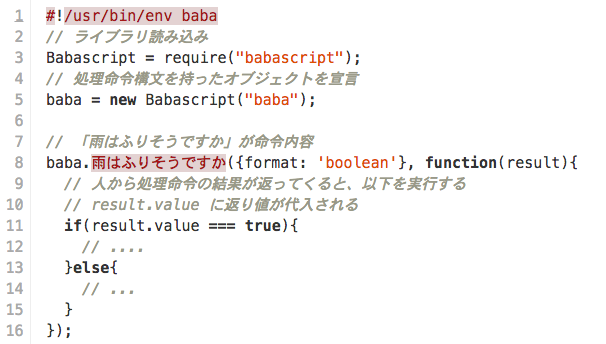
\includegraphics[width=70mm, bb=0 0 606 344]{images/basic.png}
  }
  \caption{Babascriptプログラム例}
  \label{script_01}
\end{figure}

\begin{figure}[!h]  
  \centering
  \fbox{
    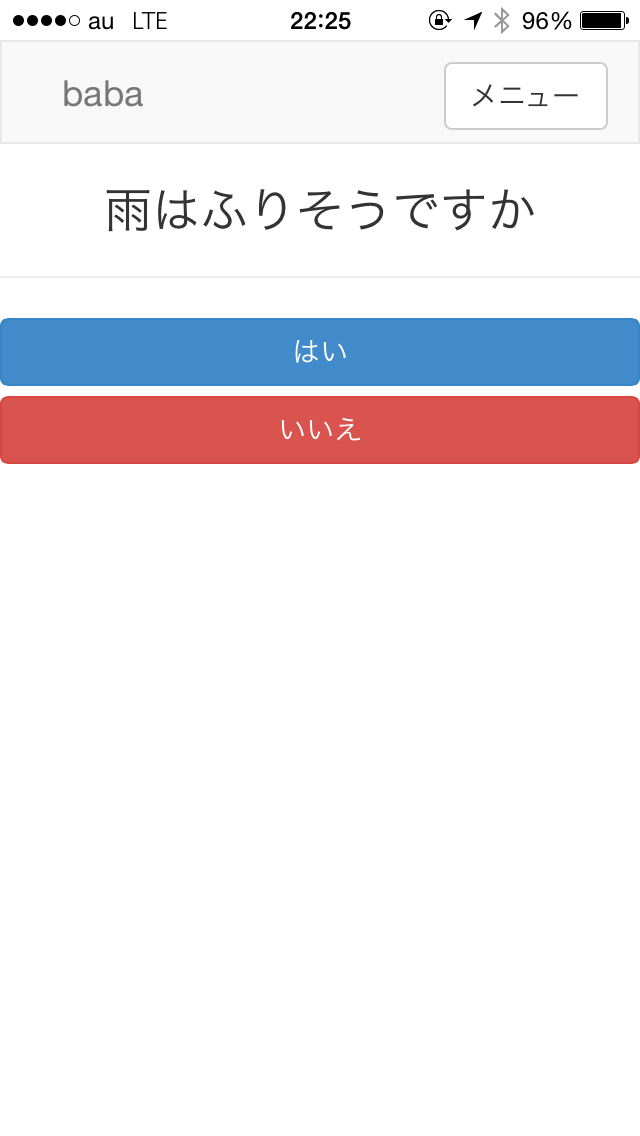
\includegraphics[width=44mm, bb=0 0 640 1136]{images/format_01.png}
  }
  \caption{Babascript Clientインタフェース}
  \label{webapp-interface}
\end{figure}

\section{BabaScriptプログラミング環境}
BabaScriptプログラミング環境は、人に対する処理命令を記述するためのBabascriptと、処理命令を受け取り、返り値を返すことのできるBabascript Clientから成り立つ。  

\subsection{Babascript}

Babascriptは、Javascript(V8 JavaScript Engine\footnote{https://code.google.com/p/v8/})上に実装された、人に対して処理命令を送る機能に特化したDSL(Domain Specific Language)である。
図\ref{script_01}のようなプログラムによって、人に処理命令を送ることができる。
Babascriptは、通常の関数を実行しているのと同じようなシンプルな記法で、人力処理のための記述を実現する。
% ここかく

\subsubsection{基本仕様}

Babascriptでは、定義されていないメソッドが実行されると、エラーを返さずに、人への命令構文として解釈する。
定義されていないメソッドは全て人への命令として実行され、人に通知される。
例えば、「toString」や「call」等のメソッドは、javascriptにおいてはほぼすべてのオブジェクトが持つメソッドだ。
一方で、「clean\_up\_your\_room」や「bake\_bread」のようなメソッドは定義しない限りは存在しないメソッドである。
Babascriptは、後者に該当する、定義されていないメソッドをエラーとして評価せず、人への命令構文として評価する。

人への命令構文として評価されたメソッドは、そのメソッド名と引数を元にしたタスク情報を生成し、Babascript Clientへと送信する。
この際、メソッド名部分がユーザに命令として提示される文となる。
メソッド名が自由に設定できるため、内容は命令文ではなく、質問のようなものもあり得るが、本研究では文章としては命令ではないものも統一して命令と呼ぶ。
人への命令構文の第一引数にはオプション情報としてオブジェクトを、第二引数には人力処理の実行後に実行するコールバック関数を指定する。
この際、コールバック関数が省略されると、タスク情報のみをBabascript Clientに通知する。

命令の実行結果をBabascript Clientから受け取ると、人への命令構文の実行を終了し、指定したコールバック関数が実行される。
コールバック関数実行時に引数として、処理に成功していれば処理実行者が入力した結果が、処理失敗であればエラー文が代入される。
人への処理命令は、通常の関数呼び出しとほぼ同じ記法で実行することができ、新たに記法を学習するといった必要がない。

人オブジェクトはインスタンス生成時にidを指定する必要がある。
人への命令構文は、このidを元に命令配信先を決定する。
例えば、id=baba に命令を送りたければ、人オブジェクト宣言時の第一引数にはbabaという文字列を指定する。
指定したidに命令が配信されるため、Babascript Client側でも同じidを指定する必要がある。
この際、指定したidに接続したクライアントが複数あった場合、後述するbroadcastオプションを指定していないと、各クライアントに順番に命令が配信される。
  
\subsubsection{オプション情報}
% ここにフォーマットについて書く
人への命令構文の第一引数には、Babascript Clientに伝送したい情報の入ったオブジェクトをオプション情報として与える。
例えば、返り値のフォーマットを指定するオプションが考えられる。
現在対応しているフォーマットはBoolean,String,Int,Listの4つが存在する。
例えば、Booleanを指定すれば、処理実行者にはtrueとfalseのどちらかを選択するインタフェースが提示される。

Listを返り値のフォーマットとして指定する場合のプログラム例は図\ref{script_02}の通りである。
フォーマット情報以外にも、選択肢の候補情報などをオプション情報として付加する。

% ここも考えなおし
% gistにして画像貼る
\begin{figure}[!h]  
  \centering
  \fbox{
    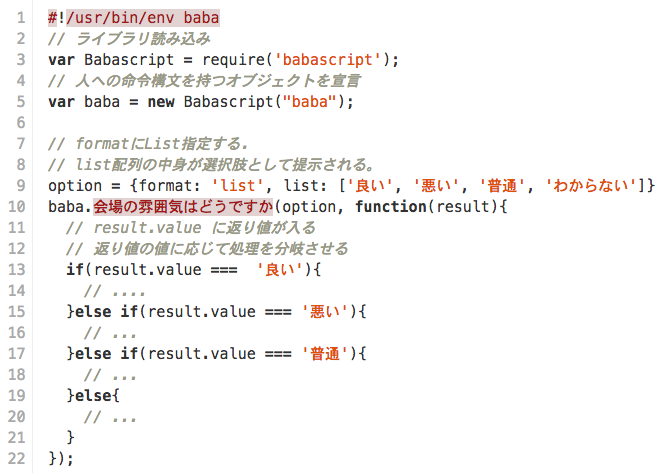
\includegraphics[width=70mm, bb=0 0 664 473]{images/list_format.png}
  }
  \caption{オプション情報例(List)}
  \label{script_02}
\end{figure}
% \begin{lstlisting}[caption=オプション情報例(List), label=script_02]
% #!/usr/bin/env baba

% Babascript = require("babascript");
% baba = new Babascript("baba");
% sho = new Babascript("sho");
% opitons = {
%   format: "list"
%   list: ["寒い", "普通", "暑い"]
% };
% baba. 部屋の温度はどうですか(options, function(result){
%   if(result.value === "寒い"){
%     sho. 部屋の温度を上げてください();
%   }else if(result.value === "暑い"){
%     sho. 部屋の温度を下げてください();
%   }
%   process.exit();
% });

% \end{lstlisting}

% 考えなおし
特別なオプション情報として、broadcastオプションが存在する。
broadcastオプションを付与することで、指定したIDに接続する全てのクライアントへと命令を配信し、指定した数の返り値を得られるまで待機し、コールバック関数を実行する。
broadcastオプションは、個人ではなく、特定のグループへの命令を想定した実装となっている。
例えば、所属研究室のメンバーに処理命令を送り、必要な数の返り値を得たら実行を終了する、といった用途に使うことが出来る。

\subsection{Babasciript Client}

Babascript Clientは、Babascriptからの命令を受け取り、値を返すためのスマートフォン向けwebアプリケーションである。
Babascriptとの通信を担うサービス部分と、返り値の入力等を担うインタフェース部分から構成される。

\subsubsection{サービス}
サービス部分では、主にBabascriptとの通信をおこなっている。
命令受信のイベントに対してコールバック関数を指定することで、処理命令を受け取ることができる。
基本的な利用方法は、図\ref{client_library}に示す。

% 書き直し
% gistにして画像貼る
\begin{figure}[!h]  
  \centering
  \fbox{
    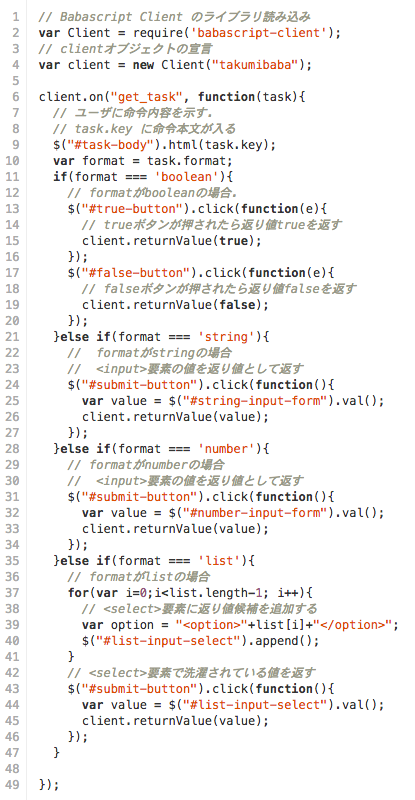
\includegraphics[width=70mm, bb=0 0 415 800]{images/client_library_image.png}
  }
  \caption{Babascript Client サービス部分のプログラム例}
  \label{client_library}
\end{figure}

クライアントオブジェクトの宣言時、IDを指定することによって、指定IDに対して処理命令が発行された際にタスクを受信することができる。
また、クライアントオブジェクトが持つreturnValueメソッドを利用することで、返り値を命令発行元に返すことができる。

サービス部分は、インタフェース部分とは分離した実装となっている。
本論文においては後述のスマートフォン向けWebアプリケーションとしてインタフェース部分を実装したが、サービス部分はWebアプリケーション以外にも適応可能である。

\subsubsection{Webアプリケーション}
% もっと詳しく

送られてきた命令内容をユーザに提示するためのインタフェースとして、スマートフォン向けWebアプリケーションを実装した。
図\ref{webapp-interface}のような画面を持つ。

Babascriptからの命令を受け取ると、インタフェースが変化し、命令内容と指定されたフォーマットに沿ったフォームをユーザに提示する。
例えば、フォーマットにBooleanを指定していた場合、ユーザには true ボタンと false ボタンが提示され、どちらかを押すと、その結果が返り値としてプログラムに返される。
Boolean以外には、String、Number、Listに対応している。
StringとNumberであれば、文字・数字の入力フォームと投稿ボタンが提示され、投稿ボタンを押した際にフォームに入力されていた内容が返り値としてプログラムに返される。
Listであれば、選択フォームと投稿ボタンが提示され、同様に、選択していた要素が返り値としてプログラムに返される。
フォーマットが指定されていない場合は、Booleanのインタフェースを提示する。

\section{実装}

上記システムは全てJavaScriptで実装した。\\
BabascriptはJavaScriptのサーバサイド実行環境であるNode.js上で動作する。
また、Babascript ClientはWebブラウザ上及びNode.js上で動作する。

全体図は図\ref{system}のとおりだ。

\begin{figure}[h]
  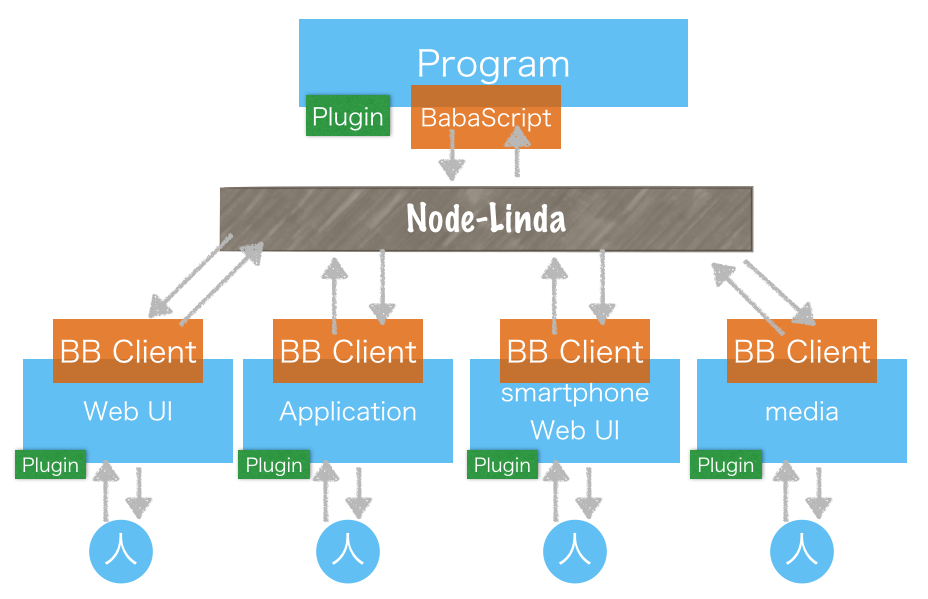
\includegraphics[width=83mm, bb=0 0 928 599]{./images/system.png}
  \caption{システム全体図}  
  \label{system}
\end{figure}

BabascriptとBabascript Client間の通信を実現するために、Node-Linda\cite{nodelinda}を利用した。
Node-Lindaは、Linda\cite{linda}モデルを拡張し、socket.io\footnote{http://socket.io}上に実装したものである。

\subsection{処理の流れ}

Babascriptは、以下のような流れで人への命令構文が実行される。

\begin{enumerate}
  \item 人への命令構文を実行する
  \item 命令がNode-Lindaサーバを経由してクライアントへと配信される
  \item 命令を受け取ったクライアントがユーザに処理を促す
  \item 命令実行者が、処理結果を入力する
  \item Node-Lindaサーバを経由して実行元プログラムに入力された処理結果が送信される
  \item プログラム側で指定されたコールバック関数が実行され、処理が継続される
\end{enumerate}

\subsection{タスク情報の構成}

人への処理命令構文の実行によってタスク情報が生成される。
このタスク情報は、図\ref{task}のようなjsonオブジェクトとなる。

\begin{figure}[!h]
  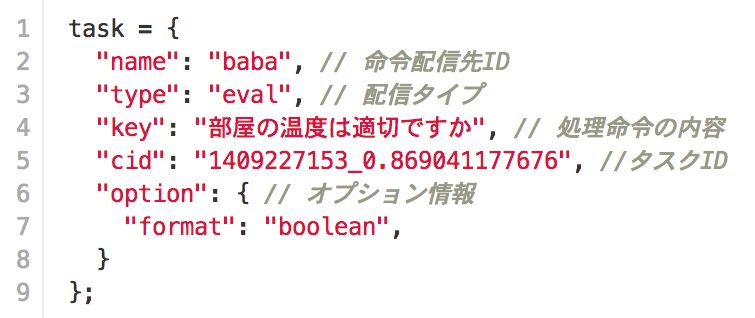
\includegraphics[width=83mm, bb=0 0 755 318]{./images/task.png}
  \caption{タスクのJSONオブジェクト}  
  \label{task}
\end{figure}

\section{応用例}

以下のような応用が考えられる。

\subsection{仕事のプログラム化}

人への命令がプログラムとして記述可能になることで、仕事をプログラム化することができると考える。
人の仕事は、例えば、マニュアルのような形で記述されることが多い。
マニュアルはどのように行動すべきかが構造的に記述された手順書であり、「Aという条件の時にはBの処理を実行する」といったことが文章として記述されていることが多い。
コンピュータにとっての手順書であるプログラムとは類似点多いと言え、プログラムに変換可能であると考える。

プログラム化して実行できるようにすることで、仕事における状態をプログラムで管理することができる。
状態を可能な限りプログラムで管理し、経験や知識によって可能な条件判断などもプログラム化することができれば、プログラムに指示されたことのみを実行するだけである程度の仕事を実行できると考える。
指示されたことのみを実行するだけでも良いということは、仕事の引き継ぎなどが最低限となり、人の代替をも容易にする可能性がある。
プログラム経由にすることで、詳細な実行ログや実行状況を把握することも可能である。
仕事の実行量の定量化や、状況監視、状況の可視化などに応用可能であると考える。

また、人同士がコミュニケーションを取ることなく、複数人を協調させるといったことも可能となる。
通常、複数人を協調させるためには、人同士が相談したり、上位の意思決定者が必要となる。
しかし、コミュニケーションはコストのかかるものであり、適切に行われない場合、問題が生じることもある。
意思決定をプログラムに委ねることは、複数人を効率よく協調させることに繋がるとも考えられる。

% 具体的なプログラム例

\subsection{人を使った実世界プログラミング}

人をセンサーやアクチュエータとして利用することで、人を使って実世界を操作することが可能となる。
現在のセンサーやアクチュエータでは、実世界に干渉するのには限界がある。
例えば、その場の雰囲気を数値化したり文字列化するといった、コンテキスト情報を伴ったセンシングは困難である。
しかし、人力処理を組み込むことのできる本提案手法ならば、コンテキスト情報を伴うようなセンシングであっても、実現可能である。
また、人を汎用的に利用可能なアクチュエータとして利用することもできる。

人をセンサーとして扱う手法は、Human as Sensorと呼ばれ、研究が多く存在しているが、人をアクチュエータとして利用する、Human as Actuator と言えるような事例は少なく、汎用的に使える事例はない。
両者を組み合わせることによって、既存の仕組みでは困難であったより柔軟な実世界へと干渉可能なプログラミングが可能となる。

また、本提案手法では通常のプログラムと人力処理のプログラムを混合させることができるため、
条件次第で人とコンピュータのどちらに処理させるかをプログラムが判断し、適切な方に処理させるということも可能である。

% 具体的なプログラム例

\section{考察}

本研究について、以下のように考察する。

\subsection{処理に対する人の積極的な貢献}

% 今まではコンピュータの演算を人間のために使うだけだった
% けど、むしろ、コンピュータの演算に人が合わせたほうが良いこともある
% コンピュータの意思決定に人が従い、それを援助していくような仕組みはなかった。
% プログラムは、コンピュータの能力を利用して人を支援するためのものであり、人はその恩恵を得るのみであった。
% コンピュータで実行可能であるならば、コンピュータで実行するべきである。


しかし、人にしか出来ないことも現在の技術では多く存在する。
そこで処理の実現を諦めるのではなく、コンピュータが得意なことはコンピュータが、人が得意なことは人がやるようにすれば良い。
人が積極的に処理に貢献し、人とコンピュータが相互に補完しあって処理を実行していくことで、全体的な処理の正確性の向上等に寄与する可能性も存在する。
それはまた、人にとってもメリットになりうるのではないかと考える。

\subsection{処理単位としての人}

本研究では、人は処理を命令され実行する存在となり、プログラム上においてコンピュータやセンサーと同等となる。
こういったことに対して心理的な拒否感を覚えることも考えられる。
しかし、一処理単位として扱うことは、大きなメリットでもある。
命令を実行するだけのノードであるということは、ただ処理内容を実行することにのみ集中すれば良いということだ。
ただやるべきことだけが提示され、その通りに動けば良いということは、深く考える必要がなく、楽であるということが考えられる。
もちろん、全ての処理がただ提示する通りに動けば良いものではないと考えられるが、
作業を楽にするための一つのアイデアであると言える。

\subsection{タスク実行の遅延と実行保障性}

Babascriptによる人への命令構文が実行されても、命令を受け取った人がすぐに命令に対する処理を実行し値を返すことを完全に保証することはできない。
タスク受信端末を見ていない、受信しても実行できないといった状況の場合、すぐに値を返すことはできない。
Babascriptによる人への命令構文は全て非同期実行する実装となっているため、人力処理の待ち時間に他の処理を実行させておくことが可能であるが、人力処理の実行待ちが全体の処理を遅延させる可能性は存在する。

また、労働関係にあるなど、強制力がある場合命令は実行されると考えられるが、強制力がない場合はそもそもタスクを無視するといったことも考えられる。
タスク実行に強制力がない場合は、金銭などのインセンティブを与えるといった手段によって、実行保障性を確保するといったことが考えられる。

\subsection{例外処理}

Babascriptにおいて、命令が想定する状況と現実の状況との乖離によって適切な返り値を選択・記述ができなくなるといった可能性がある。
これは、現実が刻々と変化していることなどから、完全に避ける事の出来ない問題であると考える。
この際、無理やり値を返すといった処理をしてしまうと、本来の状態とは違った判断がなされてしまう危険性がある。
命令文とは明らかに現実が異なっている場合などは、タスク実行者から例外としてプログラムに通知出来るような仕組みの実装によって、問題の解決へと繋げられると考える。

\subsection{命令内容の粒度}

Babascriptでは、人への命令構文の記述には制限がない。
そのため、命令の抽象度はプログラマに依存する。
抽象度が高すぎるメソッド名にしてしまうと、タスク実行者にとって理解しづらい文面となり得る。
例えば、「アレをする」といったような命令文の場合、タスク実行者は命令内容を理解できないと考えられる。
その結果、想定外の処理が実行され、意図しない結果を招く恐れがある。

具体的過ぎる命令は、全体の処理内容にもよるが、プログラム自体が冗長となり得る。
プログラムとタスク実行者の間のやりとりが増え、通信や待機時間などがボトルネックとなる可能性がある。
また、タスク実行者にとっても、やりとりが増えることで負担増になると考えられる。
処理ごとに異なると考えられるが、命令文は適切な抽象度に設計しなくてはならない。

% どんなタスクなら実行可能で、何が出来ないのか?

\subsection{複数命令の同時実行}

複数のプログラムから同時に一人のタスク実行者へとタスクが配信される可能性がある。
この際、異なるコンテキストにある命令が交互に配信され、タスク実行に大きな障害をもたらす可能性がある。
例えば、料理プログラムと掃除プログラムが同時に実行された場合、鍋で煮ている途中に「洗剤を投入しろ」などといった命令が配信されることが考えられる。

この問題は、全てのBabascriptプログラム中において、一人のタスク実行者は一つのプログラムからのみ、連続してタスクを受信できるような仕組みを用意することによって、解決可能であると考えられる。
また、応用アプリケーションでの実装になるが、コンテキストを明示し、どの処理系におけるタスクなのかをタスク実行者に示すといった手段によっても解決可能である。

\section{関連研究}

計算機では処理が難しいようなタスクを解決するために、人を計算資源として利用する手法はヒューマンコンピュテーション\cite{humancomputation}と呼ばれ、様々な研究が行われている。
インターネットを介して不特定多数の群衆にタスクを実行させるクラウドソーシングと組み合わせた研究事例も多く存在する。
クラウドソーシングのプラットフォームとしては、Amazon Mechanical Turk\cite{mechanicalturk}が存在する。
Barowy らは、CrowdProgrammingという概念を提唱し、プログラミング言語内においてクラウドソーシングによる計算とコンピュータによる計算の統合を実現した\cite{automan}。
Ahmad らは、Jabberwocky\cite{jabberwocky}という、ソーシャルコンピューティングのためのプログラミング環境を提案している。
Jabberwockyは、様々なクラウドソーシングプラットフォームを統合して管理できるDormouseと、Dormousとのインタラクションに特化したDog,MapReduce\footnote{http://research.google.com/archive/mapreduce.html}を人力処理に適応したManReduceから構成される。
Franklin らは、機械だけでは答えられないようなDBへのクエリに対する応答を、クラウドソーシングを用いることで返答可能にするCrowdDBを提案している\cite{crowddb}。
Morishima らは、人をデータソースとしてプログラムの中で利用する手法を提案している\cite{cylog}。
これらの研究は、人を計算資源やデータソースとしてシステムに組み込むことを想定しているが、
本研究では、計算資源やデータソースに限らず、実世界への干渉等も考慮に入れている。
また、本研究では実世界環境の操作を実現するために、家族や職場の人のような、特定の人物を対象としており、クラウドソーシング利用を前提とした既存研究とは異なる。

Dog\cite{dog}はWebアプリケーションにおけるユーザとのインタラクションの記述に特化したプログラミング言語として提案されている。
本研究も、人とのインタラクションの記述に特化したものであり、類似している。
DogはWebアプリケーションの実装時によくあるユーザとのインタラクションの記述に特化したものであるが、Babascriptはユーザをプログラムの処理ノードとして扱うことを想定している。

ユビキタスコンピューティングの研究分野においては、Human as Sensorという、人や人が持つスマートフォンをセンサーとして利用する概念も提唱されている。
PRISMは、スマートフォンを利用したセンシングプラットフォームだ\cite{prism}。
Liuらは、ソーシャルメディア上の人をセンサーとして扱ったQ\&AサービスMoboQを提案し、その検証を行った。
Human as Sensorに類する研究では、人をセンサーとして扱うことを対象としているが、本研究ではセンサーのみを対象としていない。

Chengらは、モーションプラットフォームにおけるモーターやメカニカル機構の代替として人を利用したHaptic Turkを提案している\cite{hapticturk}。
Haptic Turkはゲームでの利用に特化したものである。
本研究は、用途を限らない汎用的な仕組みとなっている。

加藤らは、人とロボット間でのタスク共有システム Sharedoを提案した\cite{sharedo}。
人とロボットのタスク実行における協調についても述べられており、本研究で指摘している
「処理実行において人とコンピュータは協調すべき」という考えと類似している。

\section{おわりに}

本論文では、プログラムに人への処理命令を組み込むことのできるプログラミング環境 Babascript を提案した。
既存の仕組みでは、プログラムから人に処理命令を送るためには、クラウドソーシングプラットフォームが必要であったり、複雑な構文の実行が必要である。
本論文の手法では、身近な特定の人物を命令実行対象とし、シンプルな記法での人への処理命令を実現した。

また、Babascriptによって実現が見込まれる応用例について言及した。
今後は、考察で述べたBabascriptの問題点についてシステムの改良などを行う。

{\scriptsize
\bibliographystyle{jwiss}
\bibliography{paper}
}

\end{document}


